%!TEX root = ../my_thesis.tex
\chapter{Results}


\section{Calcite experiment}

In this experiment we've observed the dissolution of calcite ($CaCO_3$) with water. We have decided to choose this reaction because the chemical reaction leading to the dissolution is simple. Moreover, it is abundant and geologically important material.\cite{hillner1992atomic}\cite{liang1996dissolution}

/ ADD SCHEMA of the setup

We have used our double PID feedback system and /InsertTipType. Calcite dissolution is an interesting process to observe with a high speed AFM. The whole process lasts X min which is observable with our setup. With a commercial AFM, that takes a few minutes for a raster scan, the dissolution process is hard to monitor (only a few pictures).
\begin{equation}\label{calcite}
CaCO_3(calcite) + H_20 \rightarrow Ca^{2+} + HCO_3^- + OH^- 
\end{equation}
We have mounted our calcite sample on top of the fast piezo-electrical ceramics. Also, we have stuck a plastic cover underneath the piezo for the water. THe calcite will dissolve itself with a losange pattern. It is linked to its original geometry.

We have imaged the same sample with different parameters: scan size, number of spirals and scanning time.

The Figures ~\ref{fig:cd1} to ~\ref{fig:cd6} show the evolution of the calcite. Every scan took 10 seconds over a surface of 10 $\mu m$. The scan pattern is an archimidean spiral with 50 loops. We observe the evolution of the front wave over time. After a few minutes, the water will saturate the calcite and the reaction will stop. You can redo the experiment by removing the water and adding new one afterwards.


\begin{figure}[!ht]
\centering
\minipage{0.32\textwidth}
  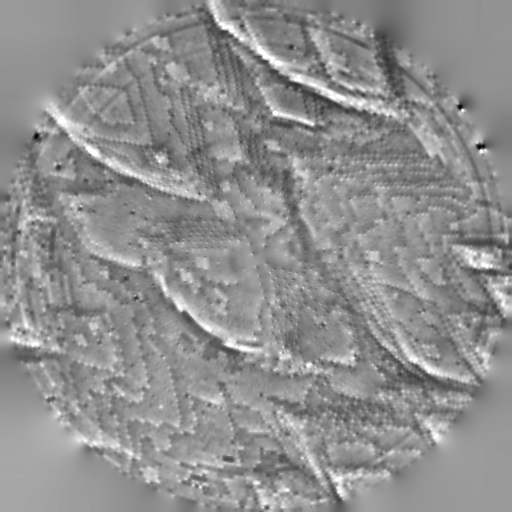
\includegraphics[width=\linewidth]{images/006_X10s50l10m_MOv2_17.png}
  \caption{}\label{fig:cd1}
\endminipage\hfill
\minipage{0.32\textwidth}
  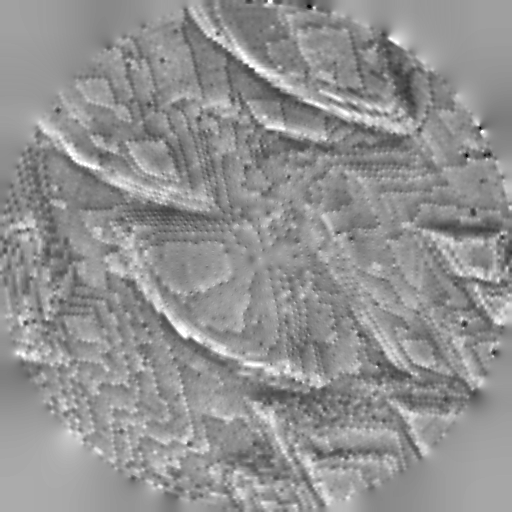
\includegraphics[width=\linewidth]{images/006_X10s50l10m_MOv2_122.png}
  \caption{A really Awesome Image}\label{fig:cd2}
\endminipage\hfill
\minipage{0.32\textwidth}%
  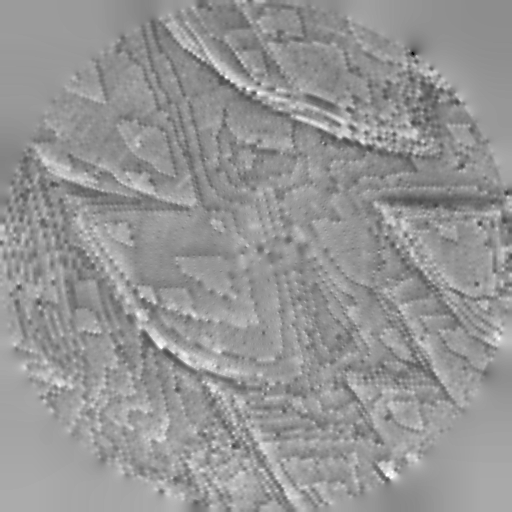
\includegraphics[width=\linewidth]{images/006_X10s50l10m_MOv2_290.png}
  \caption{A really Awesome Image}\label{fig:cd3}
\endminipage

\end{figure}


\begin{figure}[!ht]
\centering
\minipage{0.32\textwidth}
  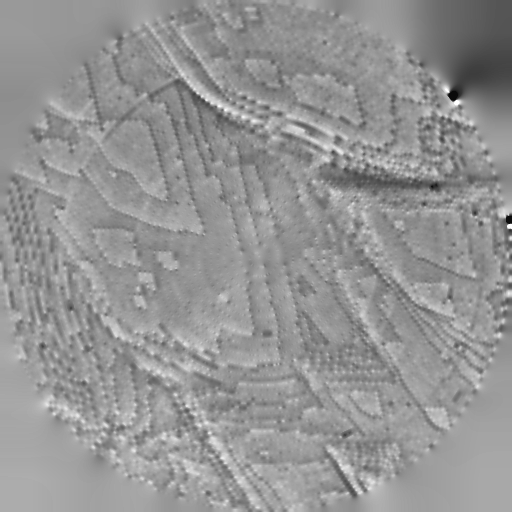
\includegraphics[width=\linewidth]{images/006_X10s50l10m_MOv2_457.png}
  \caption{A really Awesome Image}\label{fig:cd4}
\endminipage\hfill
\minipage{0.32\textwidth}
  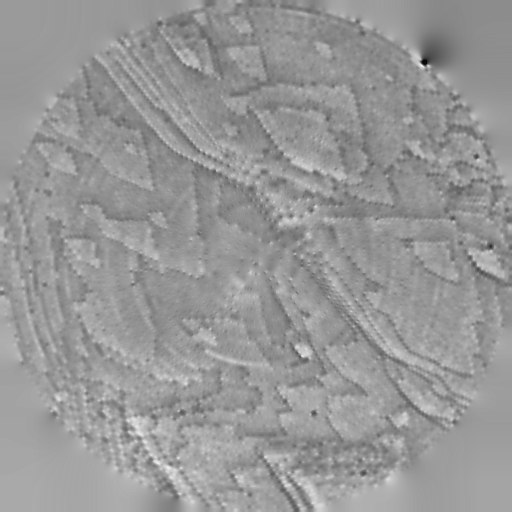
\includegraphics[width=\linewidth]{images/006_X10s50l10m_MOv2_698.png}
  \caption{A really Awesome Image}\label{fig:cd5}
\endminipage\hfill
\minipage{0.32\textwidth}%
  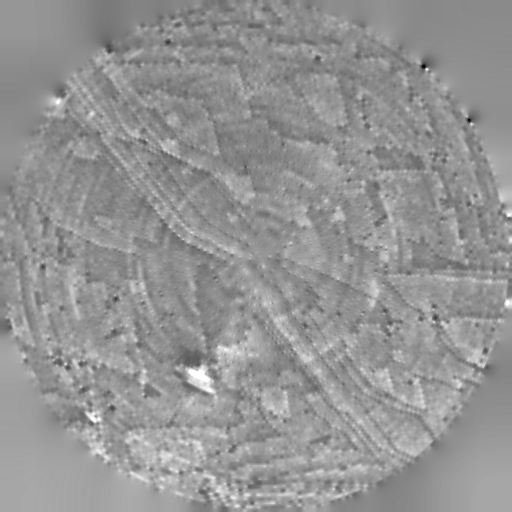
\includegraphics[width=\linewidth]{images/006_X10s50l10m_MOv2_1007.png}
  \caption{A really Awesome Image}\label{fig:cd6}
\endminipage
\end{figure}

It shows the wide range of experiments possible in the future. Inde

\section{Tilt correction}

Wavex and wavey are the x,y components of our scan pattern. The scan pattern for an Archimedean spiral is defined by the equation  ~\ref{eqarchimedean}.

\begin{equation}\label{eqarchimedean}
x(t)= \alpha \sqrt{t} cos(\beta \sqrt{t})\\
y(t)= \alpha \sqrt{t} sin(\beta \sqrt{t})
\end{equation}

We took a calibration sample to test the efficiency of our method. The size or our scan is 30 $\mu m$. We see on the figure  ~\ref{spiraheight30uv2} that the surface has a tilt. The small spikes on the curve represent the pyramids on the sample.

\begin{figure}[!ht]
\begin{minipage}[b]{0.45\linewidth}
\centering
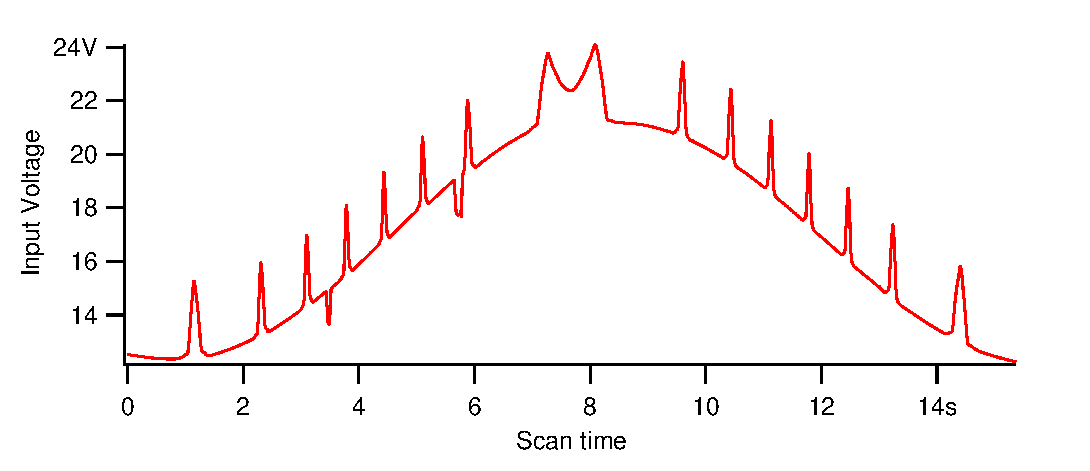
\includegraphics[width=\textwidth]{images/spiraheight30uv2.eps}
\caption{Height of the tilt correction}
\label{spiraheight30uv2}
\end{minipage}
\hspace{0.5cm}
\begin{minipage}[b]{0.45\linewidth}
\centering
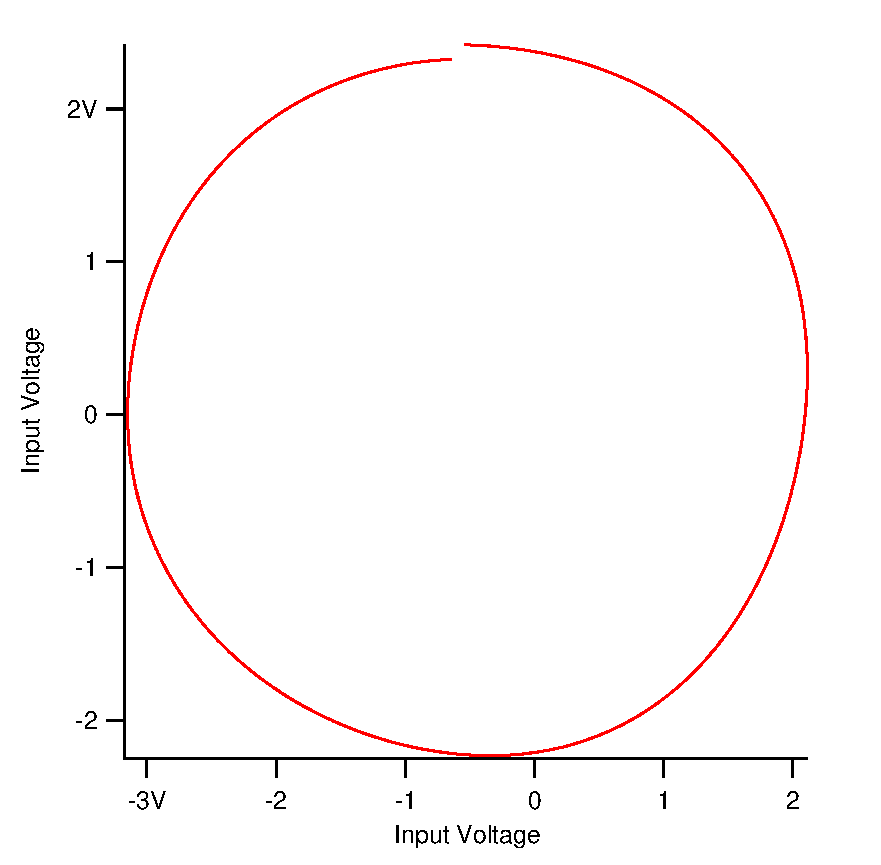
\includegraphics[width=\textwidth]{images/xsenvsysen30u.eps}
\caption{Path on the XY plane}
\label{xsenvsysen30u}
\end{minipage}
\end{figure}

Then we compute our fitting algorithm on the x,y and z data.
\begin{table}[H]
\caption{Planefit coefficients} % title of Table
\centering % used for centering table
\begin{tabular}{c c c} % centered columns (4 columns)
\hline\hline %inserts double horizontal lines
$a_1$ & $a_2$ & $a_3$ \\ [0.5ex] % inserts table 
%heading
\hline % inserts single horizontal line
-0.14615  & -0.031882 & 29.537 \\[1ex]

\hline %inserts single line
\end{tabular}
\label{table:planefit} % is used to refer this table in the text
\end{table}


The size of the scan is still 30 $\mu m$ and the spiral has 80 loops. The scan pattern we are going to send to the controller is generated with the previously computed planefit coefficients. 

\begin{figure}[H]
  \centering
  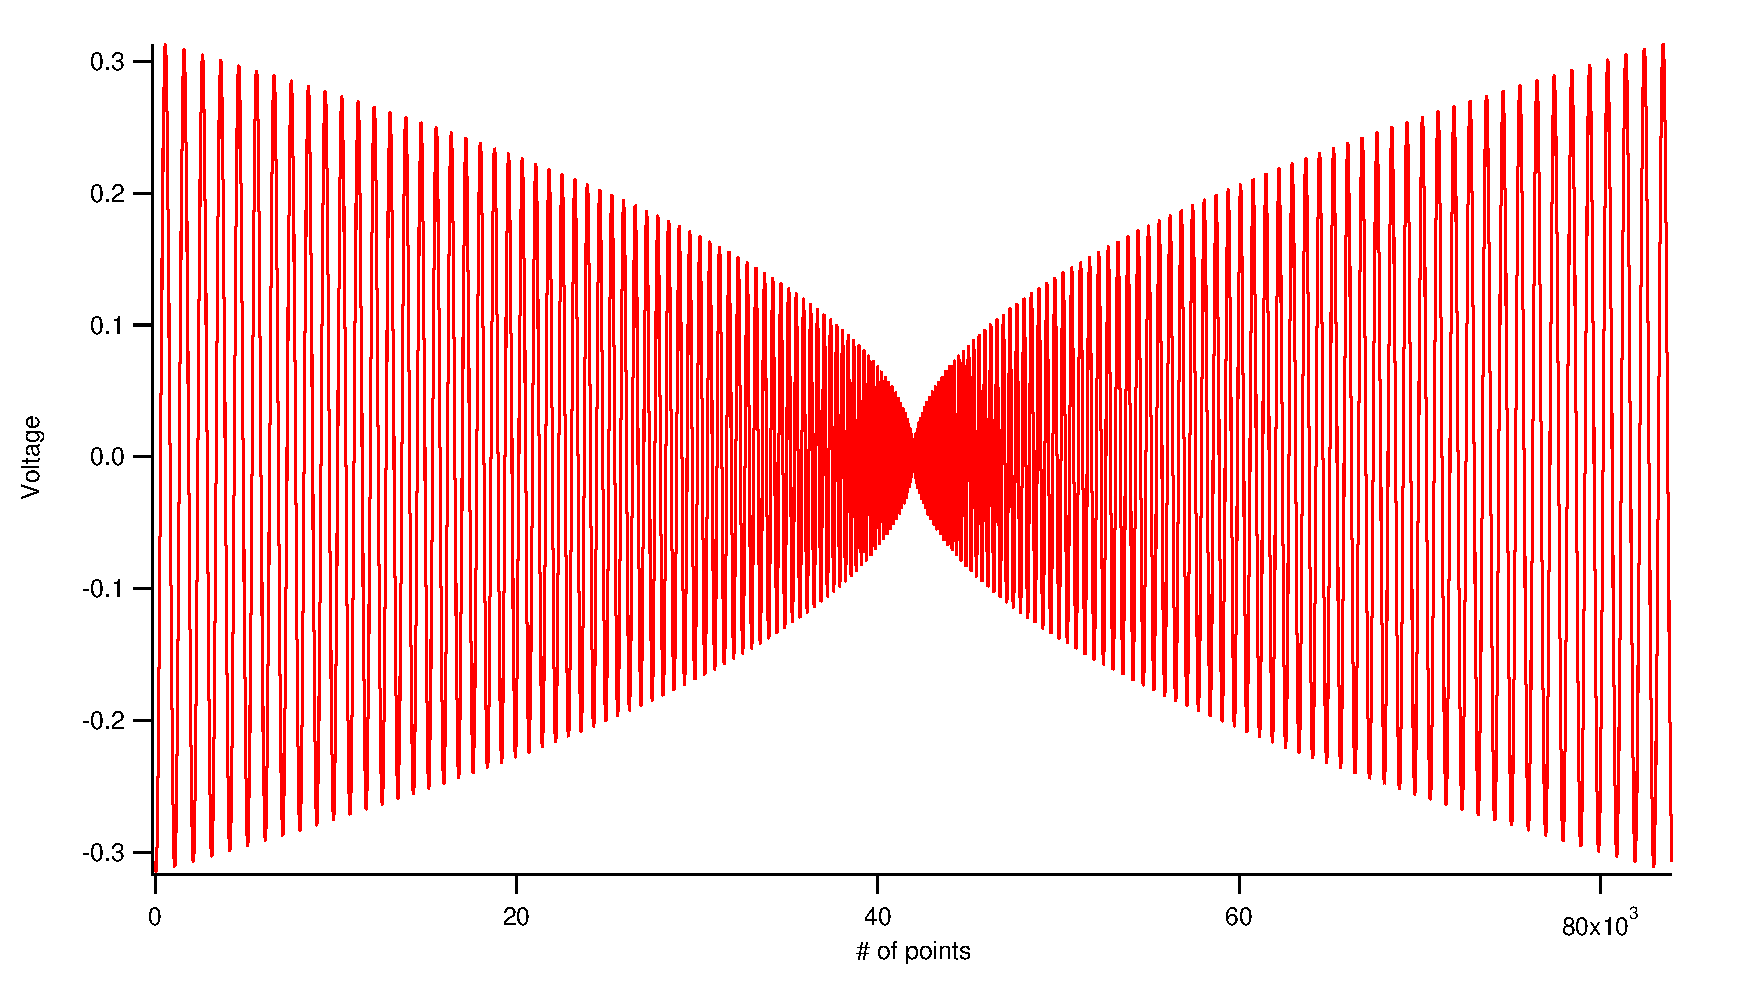
\includegraphics[scale=0.4]{images/spiralztiltout.eps}
    \caption{Input of the tilt compensation}
  \label{spiralztiltout}
\end{figure}

We have calibrated the small piezoelectric ceramic and found that a step of 5V is equal to 90 nm.
\begin{figure}[!ht]
\begin{minipage}[b]{0.45\linewidth}
\centering
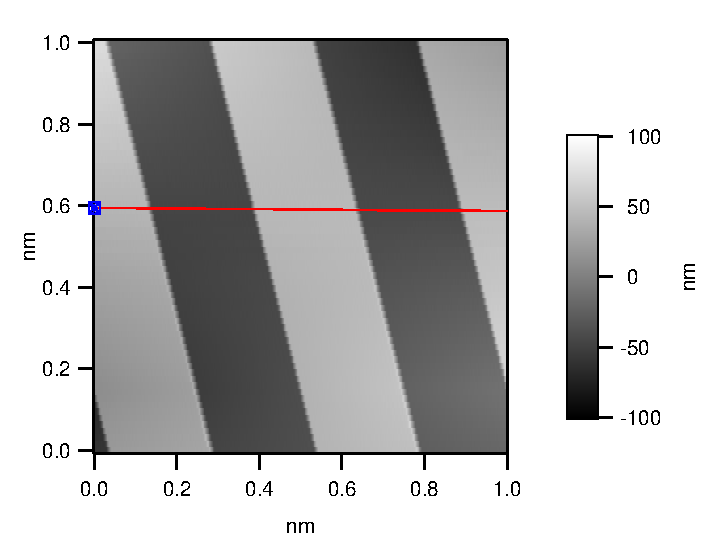
\includegraphics[width=\textwidth]{images/Calib1vPP_HeightMap.eps}
\caption{Height of the calibration}
\label{fig:figure1}
\end{minipage}
\hspace{0.5cm}
\begin{minipage}[b]{0.45\linewidth}
\centering
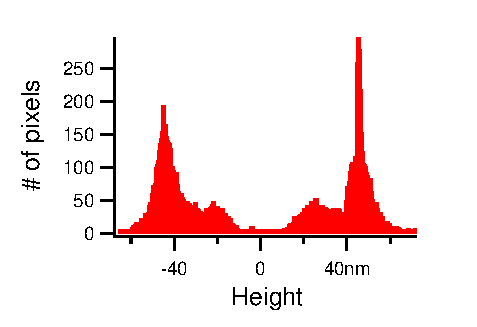
\includegraphics[width=\textwidth]{images/Calib1VppHisto.eps}
\caption{Histogram of the calibration}
\label{fig:figure2}
\end{minipage}
\end{figure}

The tilt compensation takes a load off the small fast piezoelectrical ceramics. The Figure ~\ref{spiralzfast} shows the efficiency of our method. Indeed, the fast piezo was previously saturating. The piezos was trying to reach features that are larger than his range. If we use the tilt correction, we see that our piezo has no problem reaching those features.


\begin{figure}[H]
  \centering
  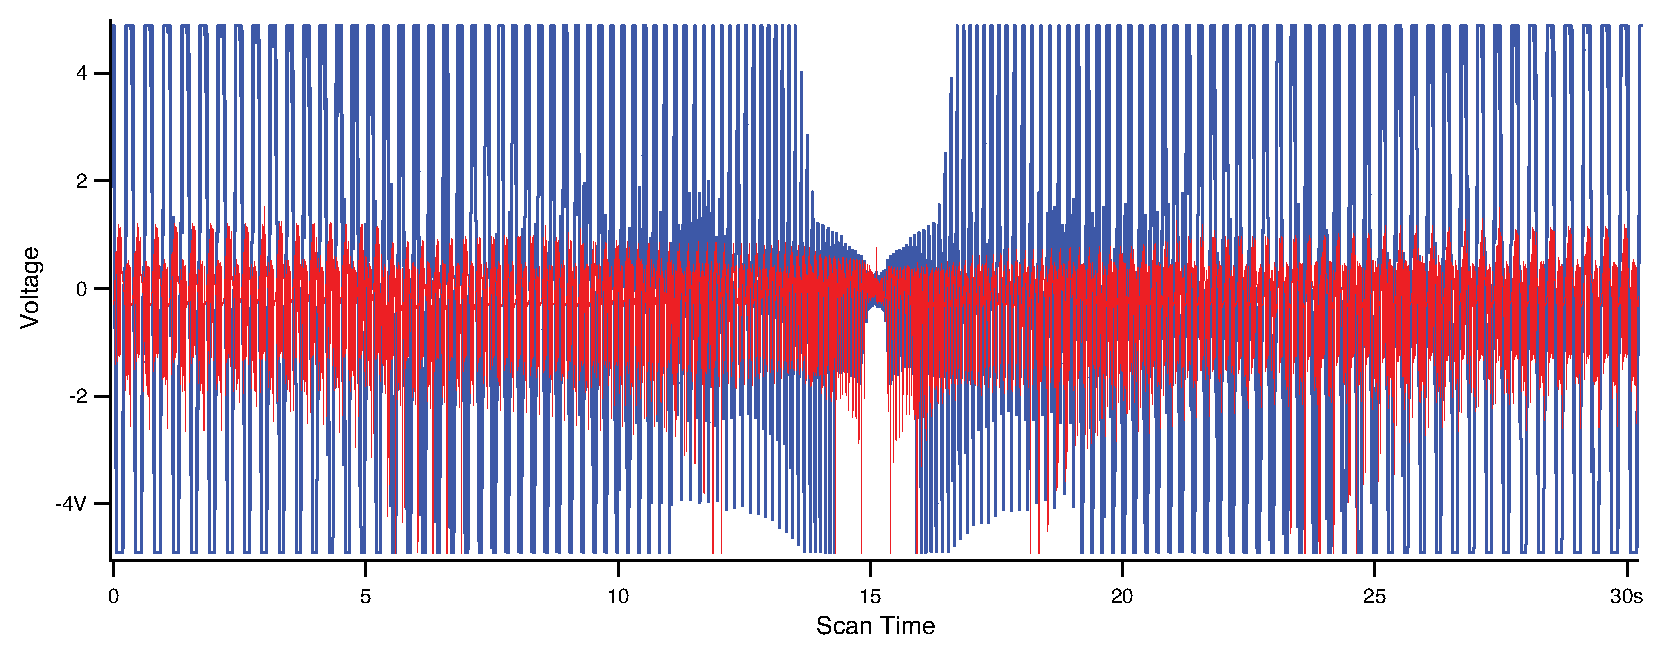
\includegraphics[scale=0.4]{images/tiltcorrectiongraph.eps}
    \caption{Output of the fast piezo}
  \label{spiralzfast}
\end{figure}

We can see the effect of the tilt correction on the following figure.

\begin{figure}[ht]
\begin{minipage}[b]{0.45\linewidth}
\centering
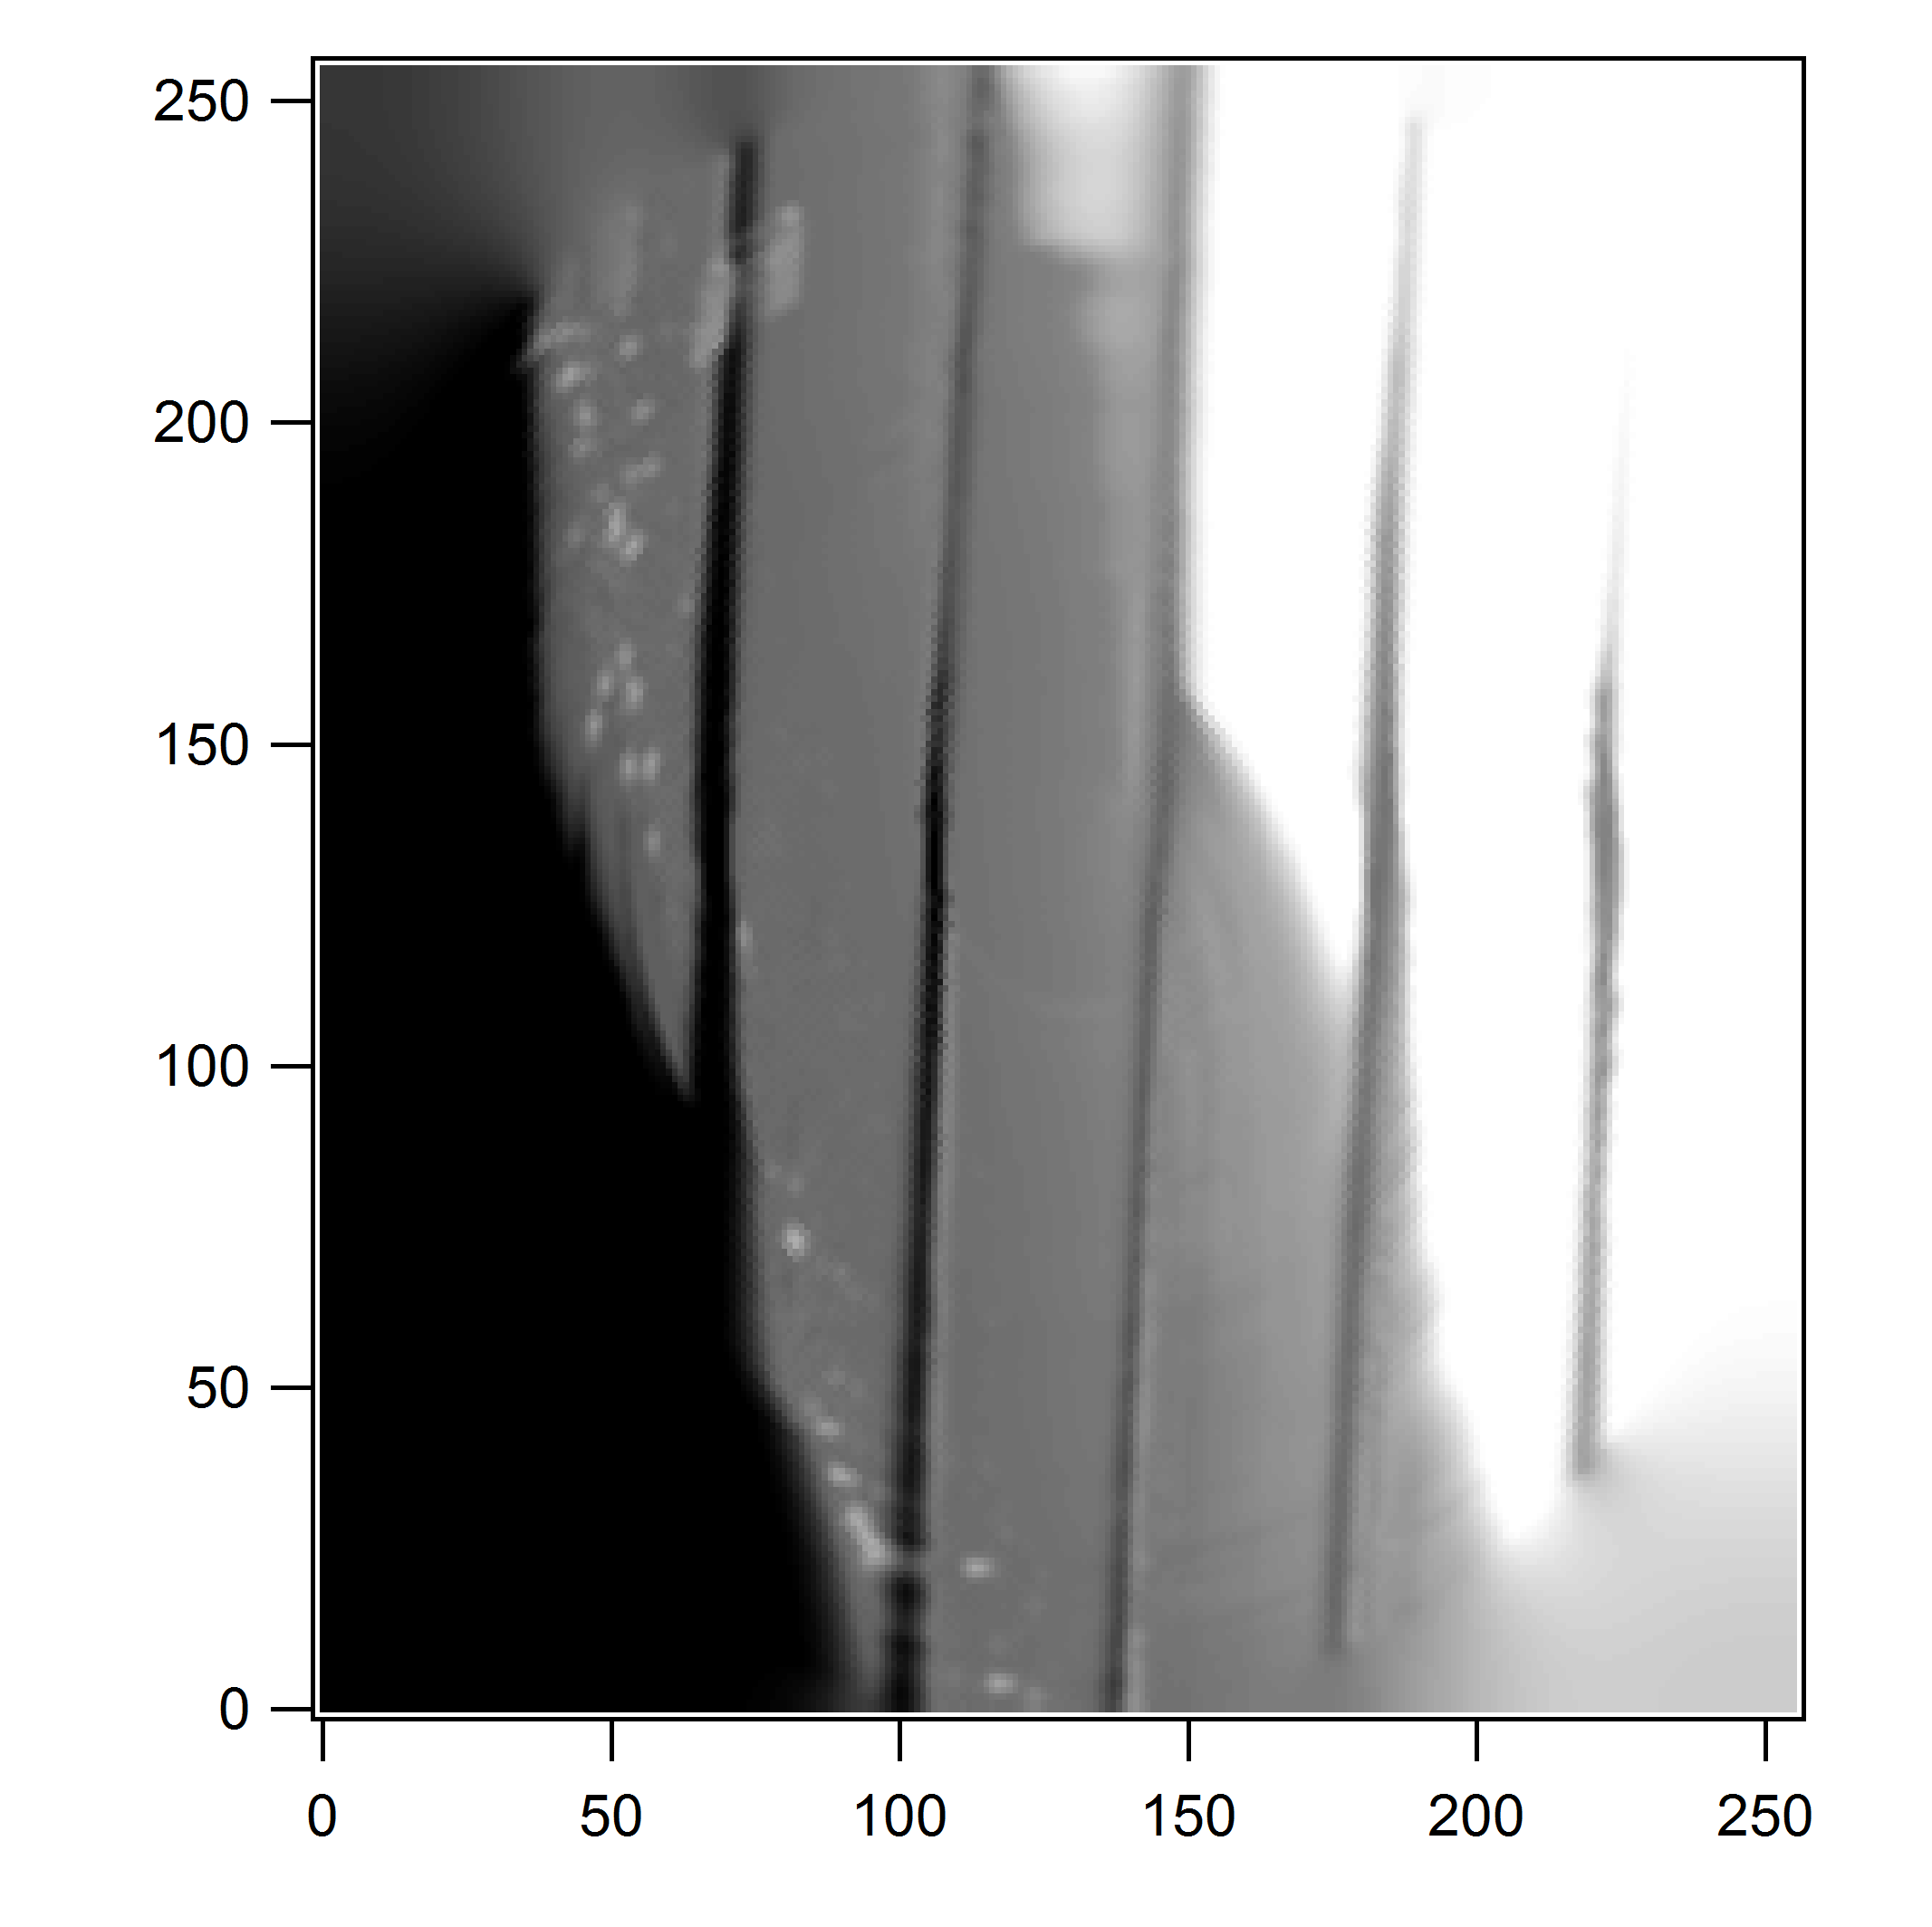
\includegraphics[width=\textwidth]{images/TiltSession0226_27.png}
\caption{Before the tilt correction}
\label{tiltbefore}
\end{minipage}
\hspace{0.5cm}
\begin{minipage}[b]{0.45\linewidth}
\centering
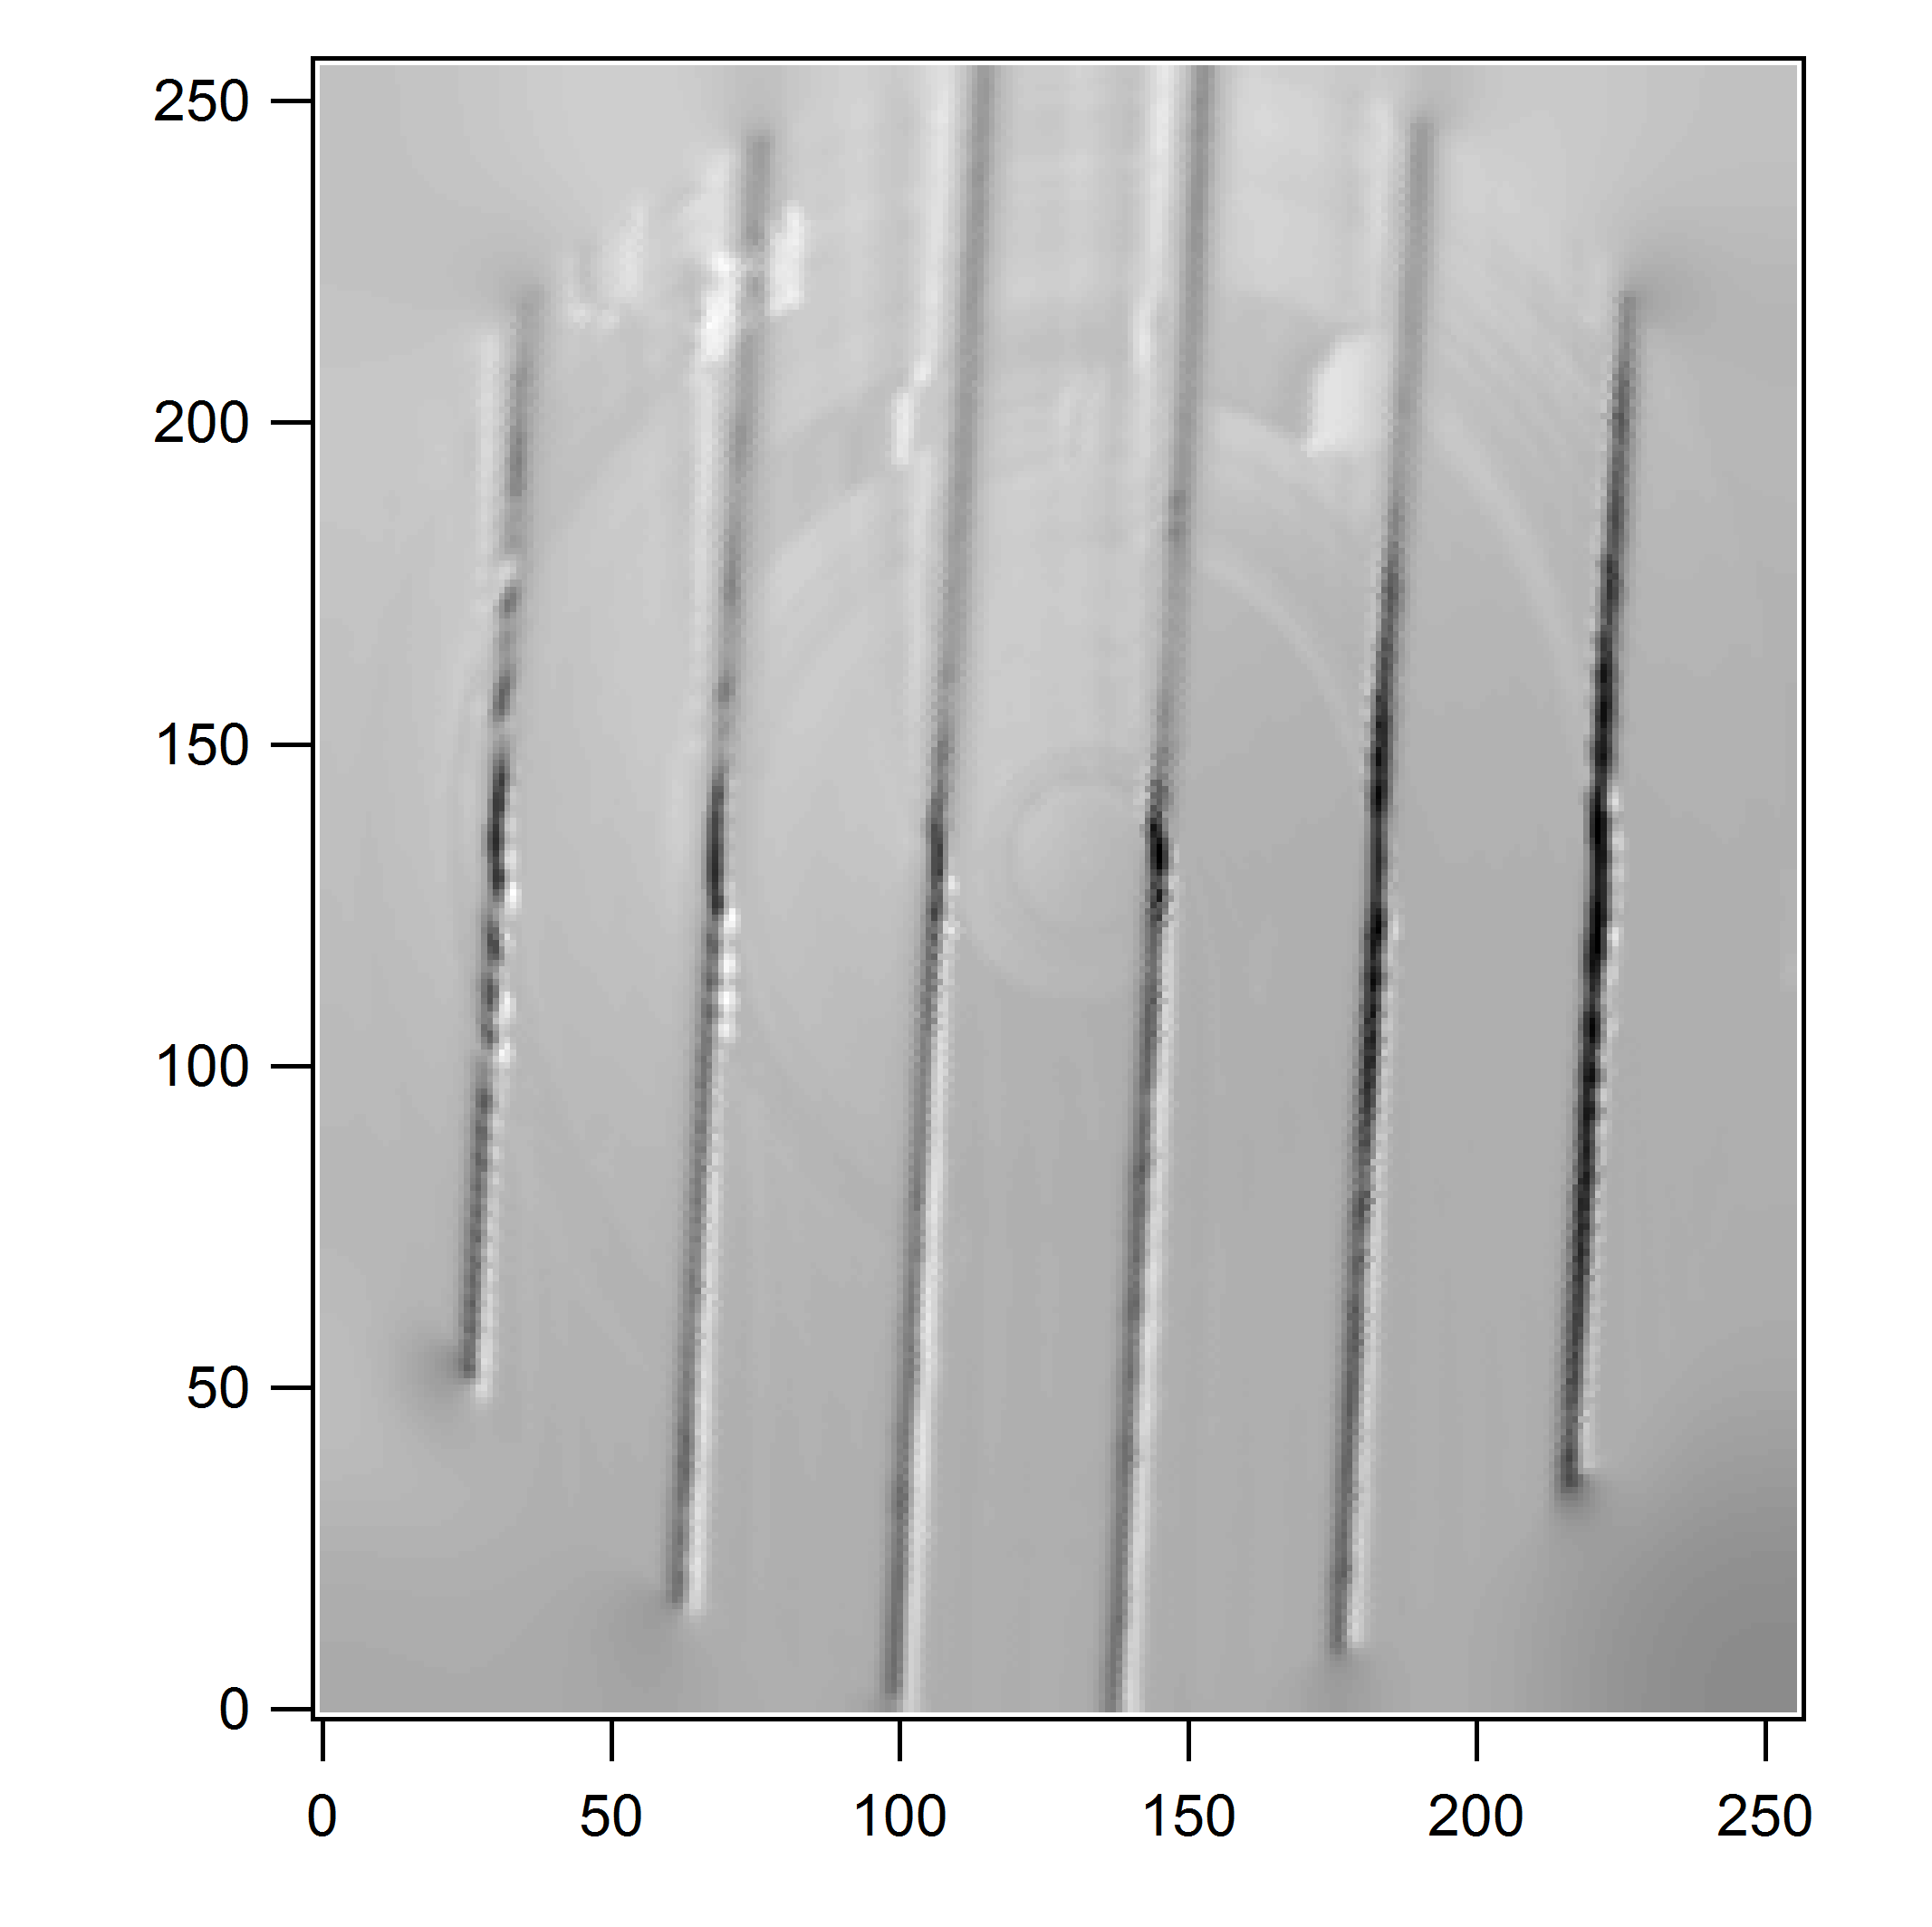
\includegraphics[width=\textwidth]{images/TiltSession0226wc_35.png}
\caption{After the tilt correction}
\label{tiltafter}
\end{minipage}
\end{figure}

